\subsection{Registration rises with atypicality and is nearly flat in lead}\label{sec:reg_rates}\label{sec:val_registration}

Figure~\ref{fig:regdeciles} gives the registration rate by decile of each
axis, with deciles cut within Nice class and filing year so that no
difference between industries or between years enters. On atypicality the
rate rises from 56.0\% in the least atypical decile to 59.1\% in the ninth
and turns down to 58.3\% in the most atypical --- a three-point climb and
a one-point turn at the top. The turn is larger in some industries than
the pooled line shows: software and electronics rises through the whole
range (51.8\% to 60.6\%), clothing dips in the middle deciles, and both
end higher than they start. On lead the range is 0.9 points with no
consistent direction: filings written in language their class was moving
toward register at nearly the same rate as filings written in language it
was leaving.

\begin{figure}[!htbp]\centering
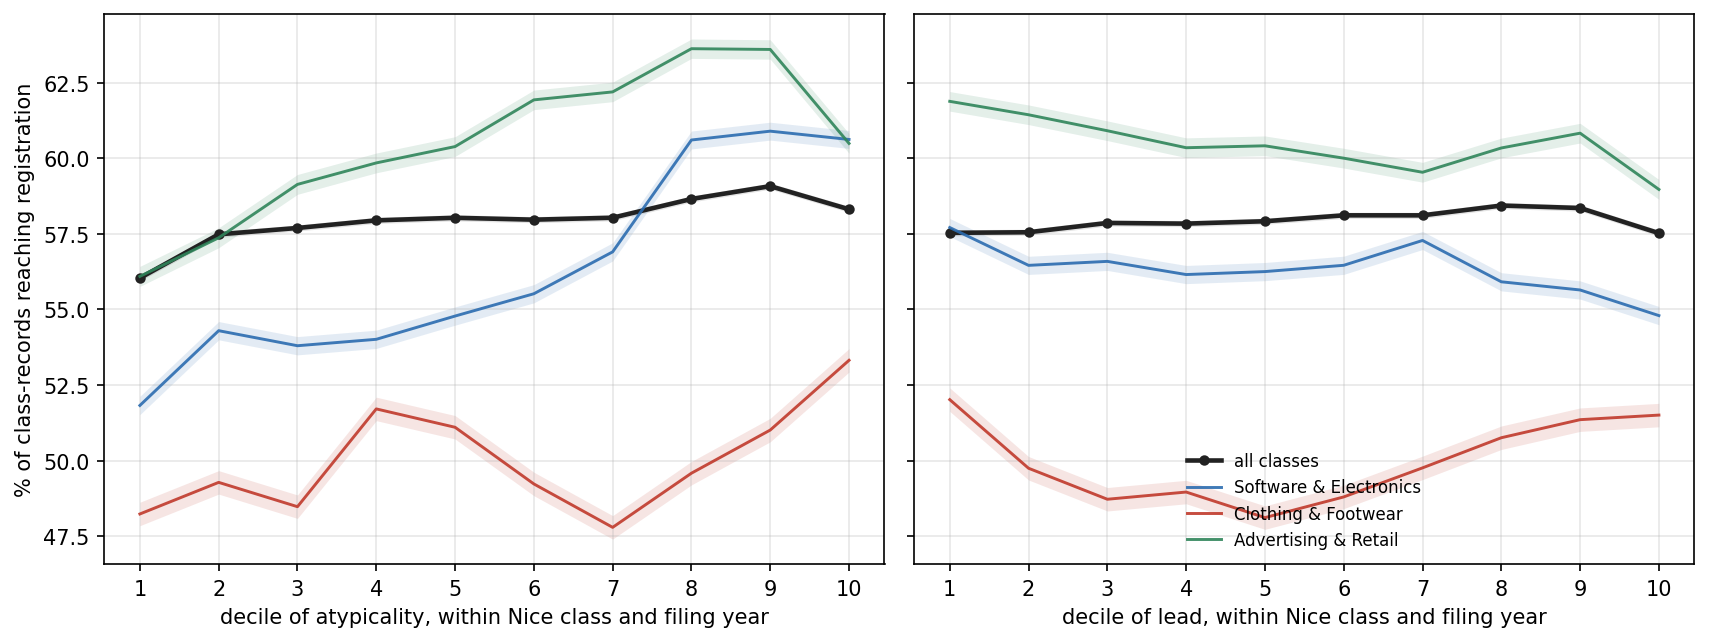
\includegraphics[width=\textwidth]{results/fig_registration_deciles.png}
\caption{Share of class-records reaching registration, filings 1995--2018,
by decile of atypicality (left) and of lead (right), deciles cut within
Nice class and filing year; $n = 9{,}024{,}532$ scored class-records. The
black line pools all 45 classes; the colored lines are three named classes.
The grey band is a 95\% binomial interval on the pooled line.}
\label{fig:regdeciles}
\end{figure}

The flatness of lead at this step has a mechanical reading worth stating:
lead is computed from the five years of filings \emph{after} the filing
date, which had not happened when the examiner acted. No participant in
prosecution could observe the quantity. Whatever small association appears
must run through correlates that were visible at the time --- the words
themselves, the industry, the drafter. Atypicality's past-facing half, by
contrast, is exactly what an examiner steeped in the class's usual language
experiences, and it is the axis registration responds to.

Figure~\ref{fig:regplane} shows the same outcome on the two surprise axes
directly, for the two largest classes: each hexagonal cell is colored by
the share of its filings that registered. The color gradient runs along
the diagonal --- from the low-surprise corner, where registration is
lowest, up through the middle of the range --- and barely across it.
Distance from the diagonal is lead; position along it is atypicality. The
plane says graphically what the deciles say numerically: the examination
step reads how far a filing sits from its class's usual language, not
which direction it faces in time.

\begin{figure}[!htbp]\centering
\includegraphics[width=\textwidth]{results/fig_registration_plane.png}
\caption{Share reaching registration across the surprise plane, filings
1995--2018 in the two largest classes. Each hexagon holds at least 50
class-records and is colored by the share of them that registered; the
dashed line is $K^- = K^+$, on which lead is zero. Cells below the line
are leading, cells above lagging.}
\label{fig:regplane}
\end{figure}

Two cautions on reading the level. First, registration is mostly a measure
of the applicant's own follow-through: of the applications that do not
register, roughly nine in ten die by inaction --- the applicant never
files the statement of use, or stops responding during prosecution --- and
only 4.3\% are removed adversarially (Table~\ref{tab:funnel}). Second,
the shape depends on how the deciles are cut. If the deciles are instead
cut on the pooled distribution, and the sample restricted to debut
filings, the atypicality curve becomes an inverse-U with a deeper
conventional tail: 46.6\% at the bottom, about 58\% in the middle,
53.4\% at the top. That version mixes in class and cohort composition; the supplementary
material reports it, with the reasons familiarity alone cannot produce
the shape. The within-cell profile of
Figure~\ref{fig:regdeciles} is the cleaner statement, and on it the
conventional tail, not the atypical one, is the penalized end. The shape
is the one audience-conformity research predicts for evaluators
\citep{Zuckerman1999, Hsu2006, Zhao2017}, here from an examiner and at
census scale; \citet{TaeuscherRothe2020} find settings where the optimum
sits off-centre.

\subsection{Examination rewards a middling specificity}\label{app:registration}

Across 3.59 million debut filings (57.6\% base rate), completion is an
inverse-U in \emph{atypicality}: it climbs from 46.6\% at the least atypical
end to about 58\% in the middle and falls back to 53.4\% at the most atypical
(Figure~\ref{fig:profiles}, panel C). The same shape appears on the
past-facing level alone, more mildly, running 54.0\% at the bottom quintile to
58.4--59.1\% in the middle and 57.7\% at the top (Figure~\ref{fig:outcomes}A).

The signed axis behaves differently. Completion on $L$ falls to a trough of
51.9\% just above the median and then rises steadily to 58.0\% at the leading
end. That trough is composition rather than timing. Lead magnitude
correlates with atypicality at $+0.31$, so the filings near zero lead are
disproportionately the low-atypicality filings, and those complete poorly
for the reason above. Splitting by atypicality confirms it: the trough is
absent in the upper three fifths and survives only in the lowest. The
signed axis still enters a linear specification strongly
(harmonized estimates in the companion paper), but monotonically rather than through an interior
peak: what curvature exists at registration belongs to how far a filing's
language sits from its category, not to which side of it the filing sat.

\begin{figure}[!htbp]\centering
\includegraphics[width=\textwidth]{results/debut_outcome_topic.png}
\caption{Outcomes for debut filings (owner's first-ever filing) across all
45 Nice classes under theme scoring, filing years 1995--2018, in quantile
bins with 95\% intervals, quantiles cut on the pooled distribution.
$n = 3{,}589{,}068$; registered subset $n = 2{,}066{,}600$. \emph{A:}
P(reached registration). \emph{B:} P(owner ever in SEC EDGAR, the
Commission's public filing system $\mid$ registration).}
\label{fig:outcomes}
\end{figure}

\begin{figure}[!htbp]\centering
\includegraphics[width=\textwidth]{results/quintile_profiles.png}
\caption{Quintile profiles for the three outcomes. \emph{A:} the share of
registrations failing the five-year proof of continued use, by lead
quintile, adjusted within Nice class and registration year with the
drafting and filer controls of Table~\ref{tab:gate_lpm}; the dashed line
is the rate for all registrations. The profile rises gently and
monotonically through the fourth quintile and then steps up: about seven
tenths of the top-to-bottom gap is the single step from the fourth
quintile to the fifth, seven times the average step below it. \emph{B:}
the share of first-time filers whose owner ever reaches SEC reporting, by
quintile of atypicality and of lead, adjusted within Nice class and filing
year with description length held. \emph{C:} raw registration rates for
debut filings in twenty bins, cut on the pooled distribution --- an
inverse-U on atypicality, and on lead a trough just above the median that
is compositional, absent once atypicality is held in its middle fifth
(dashed). Horizontal line at the pooled rate.}
\label{fig:profiles}
\end{figure}

\begin{figure}[!htbp]\centering
\includegraphics[width=0.9\textwidth]{results/fig_registration_sankey.png}
\caption{The registration step as a flow, unique serials filed 1995--2018
($n = 6{,}877{,}795$), split by counsel of record on the filing.
Represented applications reach registration at 61.9\%, self-filed at
45.6\%.}
\label{fig:sankey}
\end{figure}

The obvious objection is that unfamiliar language is simply refused more
often, so the measure recovers nothing beyond familiarity. Completion falls at
\emph{both} ends, so the most category-typical filings also complete less than
the middle, which familiarity cannot explain; and the curvature is specific to
the unsigned axis, the signed axis showing no interior peak at all.

Refiling after abandonment is itself mildly related to vocabulary position,
though not on the axis that matters here. Refiling rates are flat in
atypicality (a middle-minus-tails difference of $-0.06$pp on a 3.6\% base) but
rise with lead, from 2.6\% among the most lagging abandoned applications to
3.4\% among the most leading.

